The toolchain has been implemented in the Rust programming language
\cite{rust}.\footnote{Rust is a systems programming developed by Mozilla
Research and thousands of independent contributors from all around the world.
Rust focuses on memory safety without garbage collection, concurrency without
data races, abstractions without overhead, and stability without stagnation.} It
consists of a number of programs, and the programs are composed of a number of
stand-alone packages. The toolchain also makes use of third-party software.
Regardless of the origin, each component of the toolchain is open source. The
code written by us is distributed under the \sc{MIT} license \cite{mit} and is
available at \cite{sources}. Feedback is welcome, and contribution will be very
much appreciated.

The main programs of our toolchain are called \recorder\ and \streamer, and we
shall describe them next.

\subsection{Recorder}
\begin{figure}
  \centering
  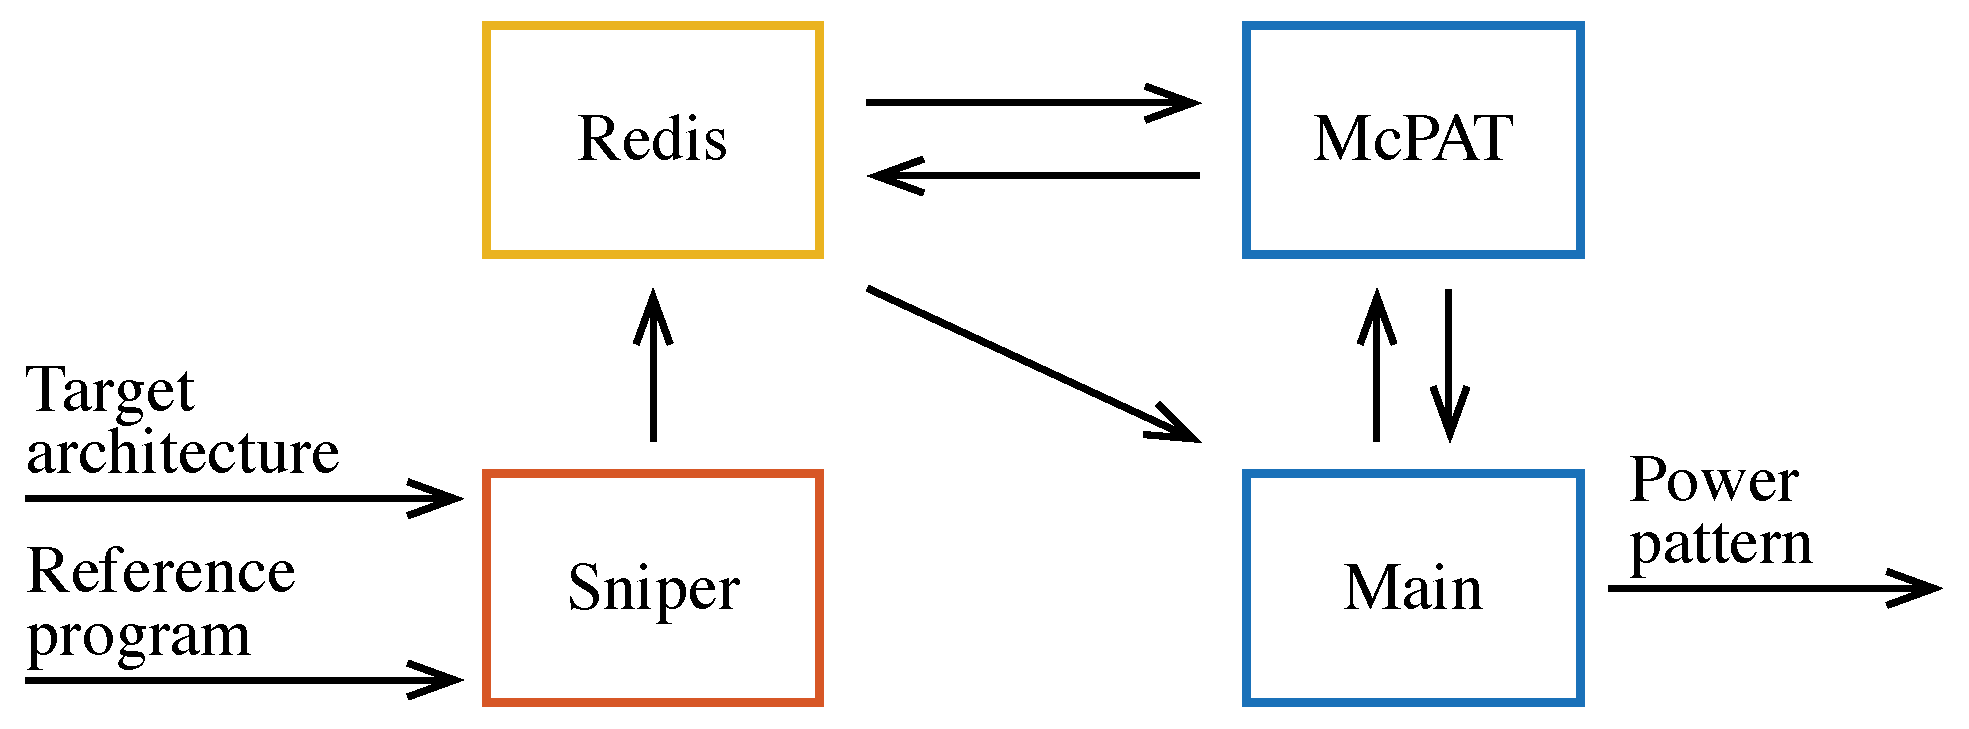
\includegraphics[width=1.0\columnwidth]{include/assets/figures/recorder.pdf}
  \caption{
    The recording infrastructure. The Recorder tool corresponds to the two blue
    boxes on the right-hand side of the figure.
  }
  \flab{recorder}
\end{figure}

\begin{table}
  \begin{threeparttable}
    \caption{Target architecture}
    \begin{tabular*}{\linewidth}{=L{70pt}l}
      \toprule
      Component    & Description \\
      \midrule
      Core         & 2660 MHz, 1.2 V \\
      L1-I/D cache & 32 KB, 4-way, LRU, private \\
      L2 cache     & 256 KB, 4-way, LRU, private \\
      L3 cache     & 8192 KB, 16-way, LRU, one per four cores \\
      \bottomrule
    \end{tabular*}
    \tlab{target}
    \begin{tablenotes}
      \item A detailed description of the target architecture can be found in
      the \texttt{nehalem.cfg} and \texttt{gainestown.cfg} configuration files
      of Sniper.
    \end{tablenotes}
  \end{threeparttable}
\end{table}
% vim: nowrap tw=0

As the name suggests, the purpose of \recorder\ is recording. More specifically,
the tool records reference workload patterns, which are needed as an input to
\streamer. The recording infrastructure is depicted in \fref{recorder}.

The performance simulator is Sniper \cite{carlson2011}.

The power simulator is \sc{McPAT} \cite{li2009}.

The key-value storage is Redis \cite{redis}.

The database is SQLite \cite{sqlite}.


\subsection{Streamer}
